\chapter{Performance Evaluation}
\label{chp:perfeval}

Bottleneck can happen in the early time of share mode. The combination of line \ref{alg:l_lts:retdlenough} and \ref{alg:l_lts:retdling} will hold downloading any piece if the uploaded amount is not enough based on the piece we have. Let say we already which piece to download from line \ref{alg:l_lts:dlrare}. In the next round, this piece is not rare anymore. Therefore, we cannot upload this piece. 

\section{Predownload}
\begin{figure}[h]
	\centering
	\includegraphics[width=\textwidth]{pics/results/dpredown_t30i30.pdf}
	\caption{Predownload success percentage}
	\label{fig:predownprecent}
\end{figure}

\begin{figure}[h]
	\centering
	\includegraphics[width=\textwidth]{pics/results/hpredown_t30i30.pdf}
	\caption{Predownload distributed time}
	\label{fig:predownhist}
\end{figure}

\begin{figure}[h]
	\centering
	\includegraphics[width=\textwidth]{pics/results/ppredown_t30i30.pdf}
	\caption{Amount of peer discovered}
	\label{fig:peeramount}
\end{figure}
\todo{From experiment \#46 500 swarm in source. 12h}
\subsection{Other piece selection}
Random : some of the piece start downloading near the end, so it can't be decided in which distribution.

Seq : 1 swarm also

\begin{figure}[h]
	\centering
	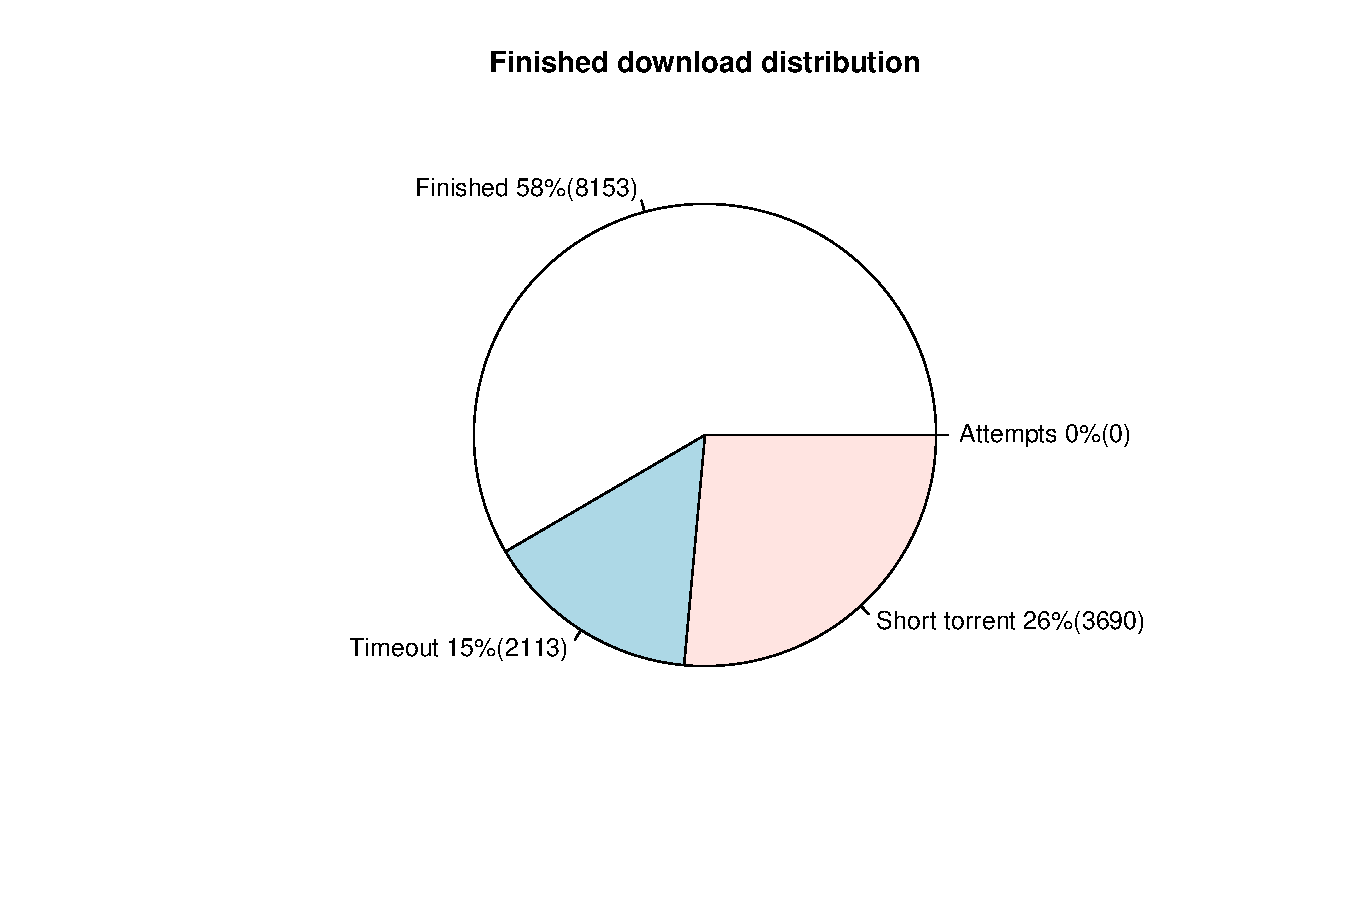
\includegraphics[width=\textwidth]{pics/results/dpredown_random.pdf}
	\caption{Predownload success percentage in random piece selection}
	\label{fig:predownprandom}
\end{figure}

\begin{figure}[h]
	\centering
	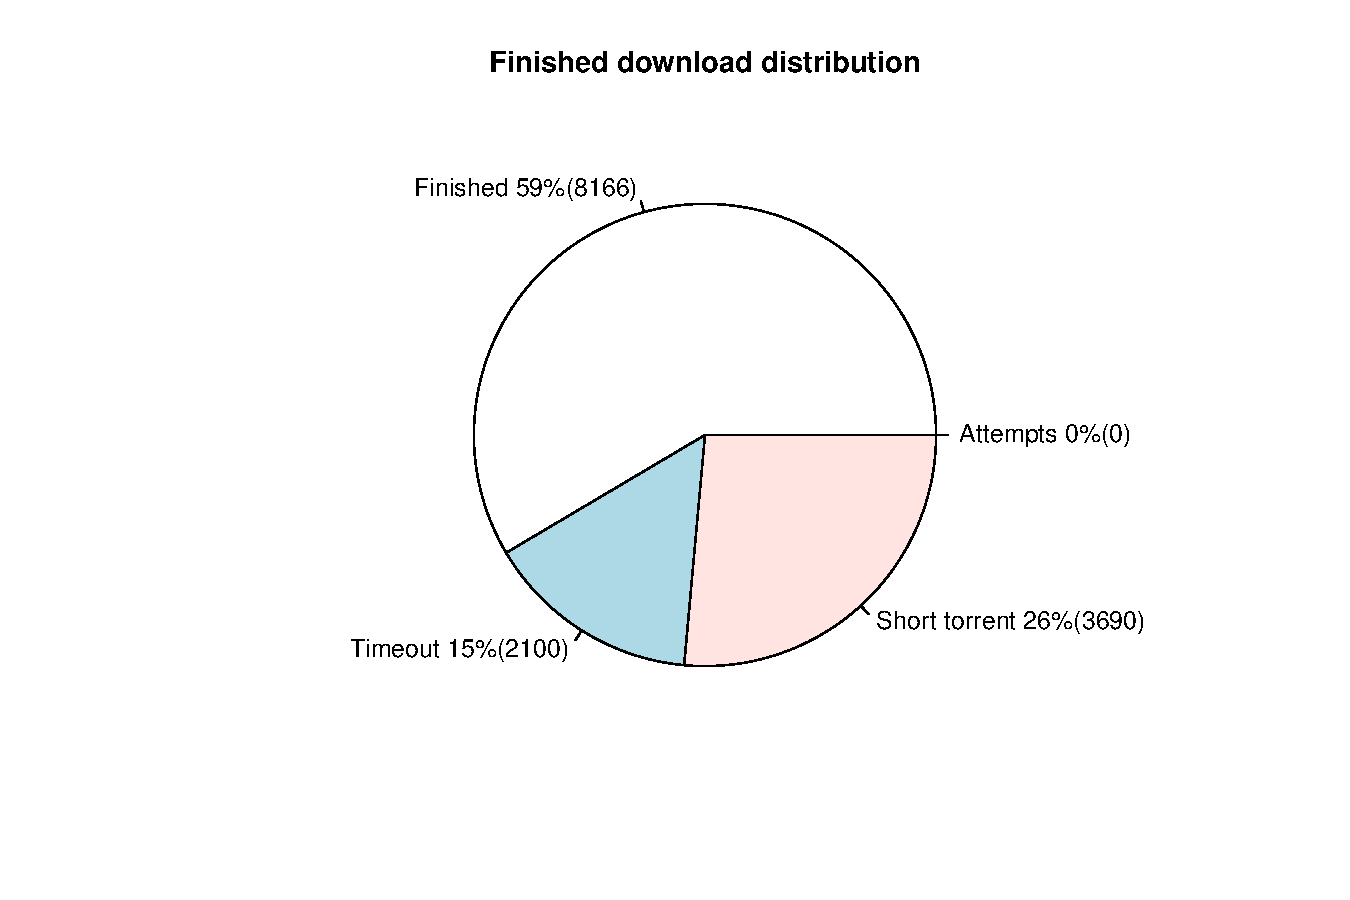
\includegraphics[width=\textwidth]{pics/results/dpredown_sequential.pdf}
	\caption{Predownload success percentage in sequential piece selection}
	\label{fig:predownpseq}
\end{figure}
\clearpage
% 100 swarm for 12, 24. 500 swarm for 24h
\section{Comparison vs old}
\begin{figure}[h]
	\begin{adjustwidth}{-2.5cm}{}
		\begin{subfigure}[t]{0.7\textwidth}
			\centering
			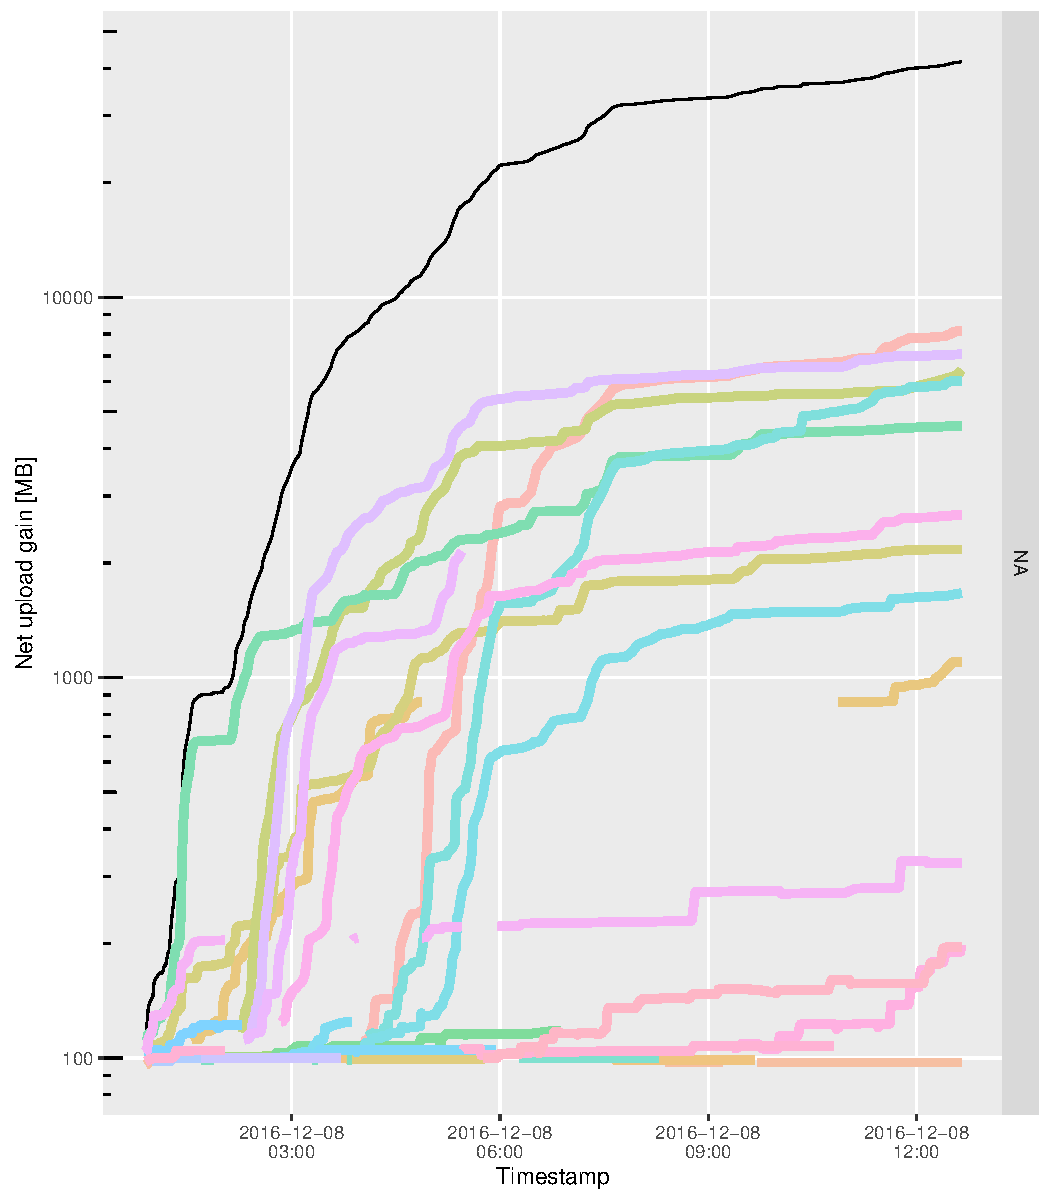
\includegraphics[width=\textwidth]{pics/results/b133.pdf}
			\caption{12 hour new experiment.}
		\end{subfigure}
		~
		\begin{subfigure}[t]{0.7\textwidth}
			\centering
			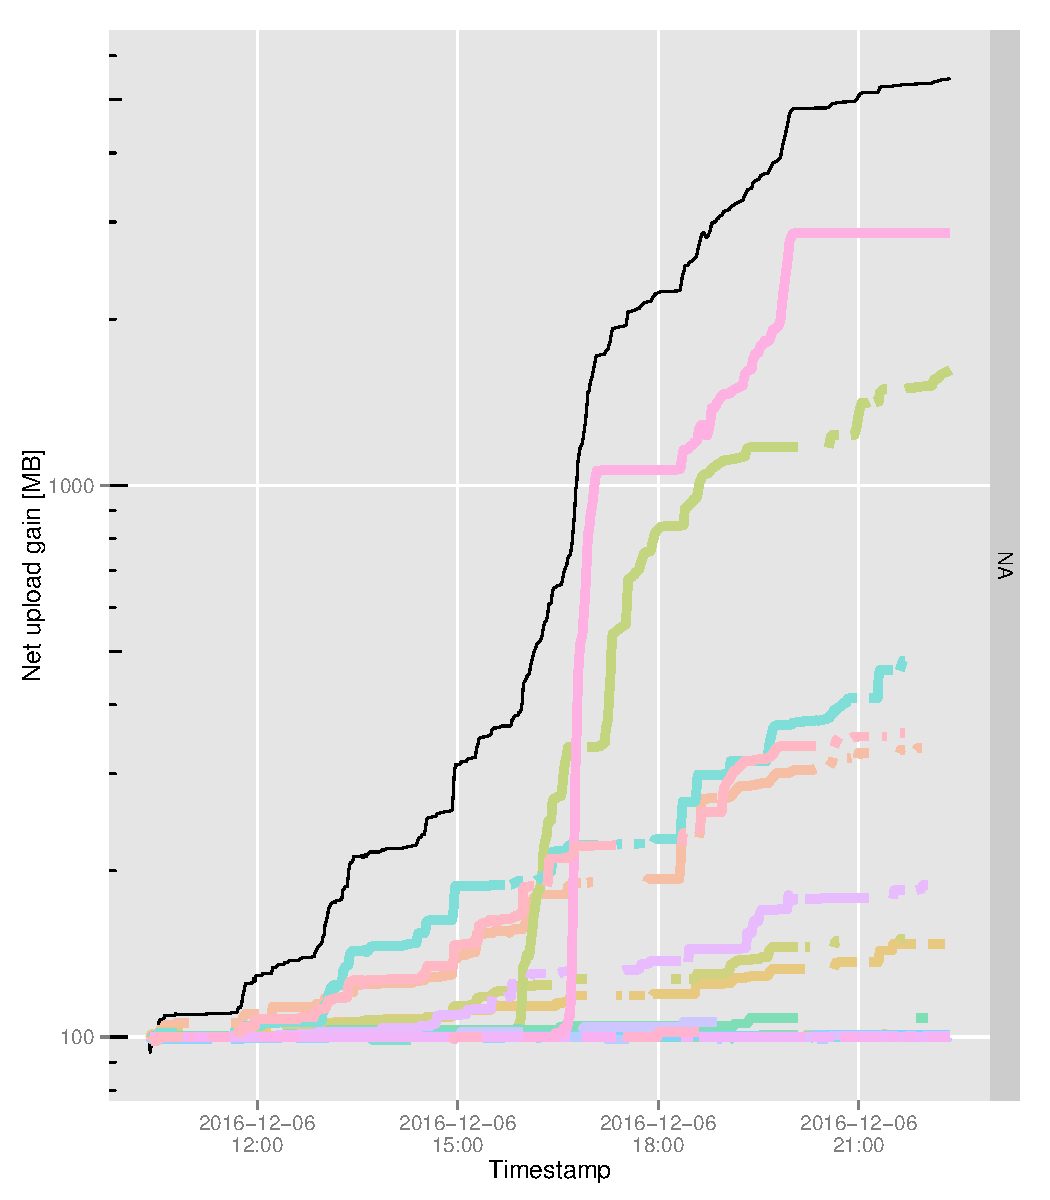
\includegraphics[width=\textwidth]{pics/results/m136.pdf}
			\caption{12 hour old experiment}
		\end{subfigure}
		\caption{New vs old experiments (run separately) result on 12 hour}
	\end{adjustwidth}
\end{figure}

\begin{figure}[h]
		\begin{adjustwidth}{-2.5cm}{}
	\begin{subfigure}[t]{0.7\textwidth}
		\centering
		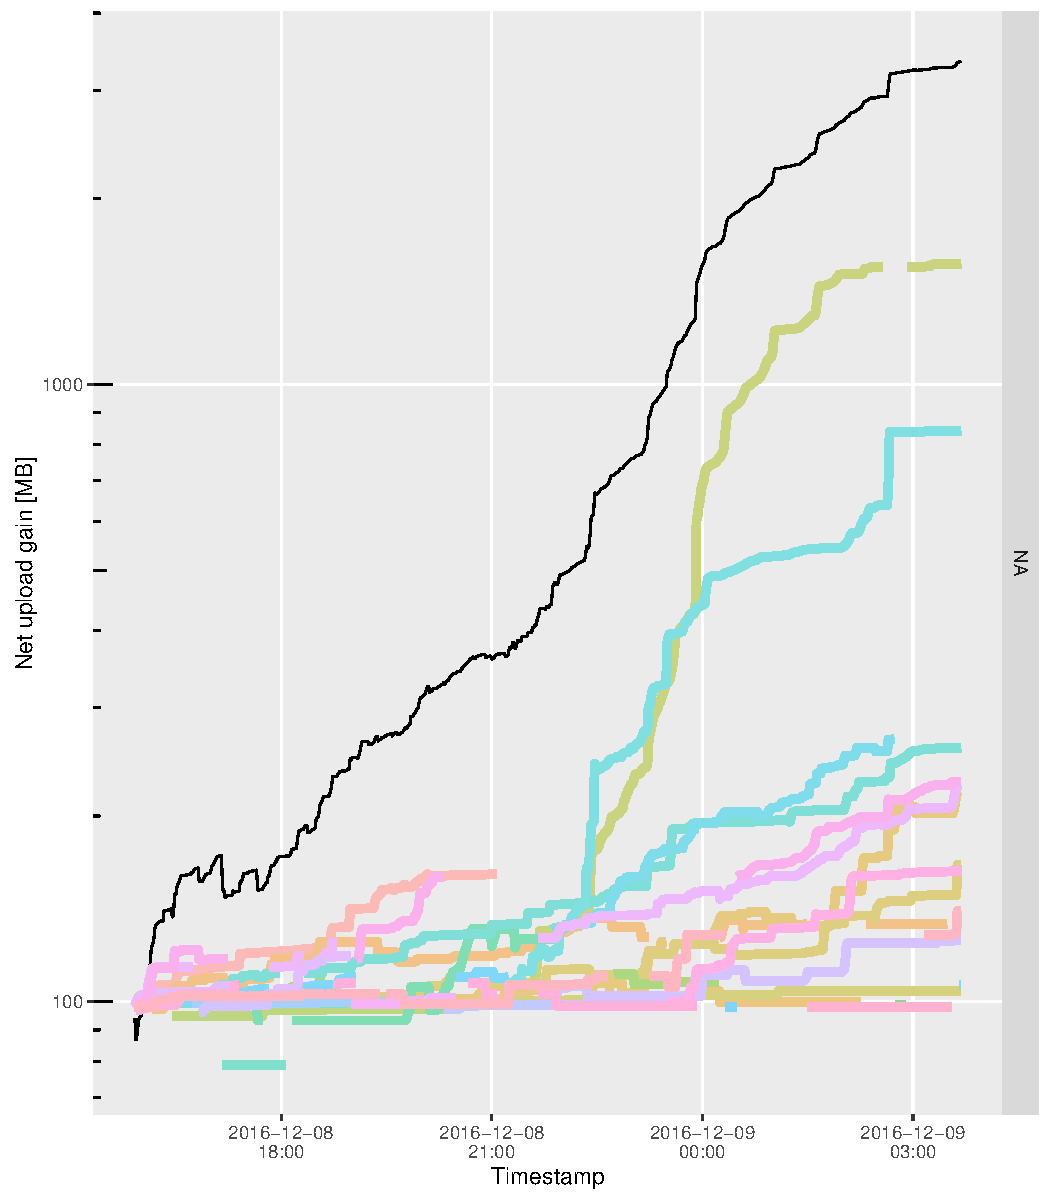
\includegraphics[width=\textwidth]{pics/results/b134.pdf}
		\caption{12 hour new experiment.}
	\end{subfigure}
	~
	\begin{subfigure}[t]{0.7\textwidth}
		\centering
		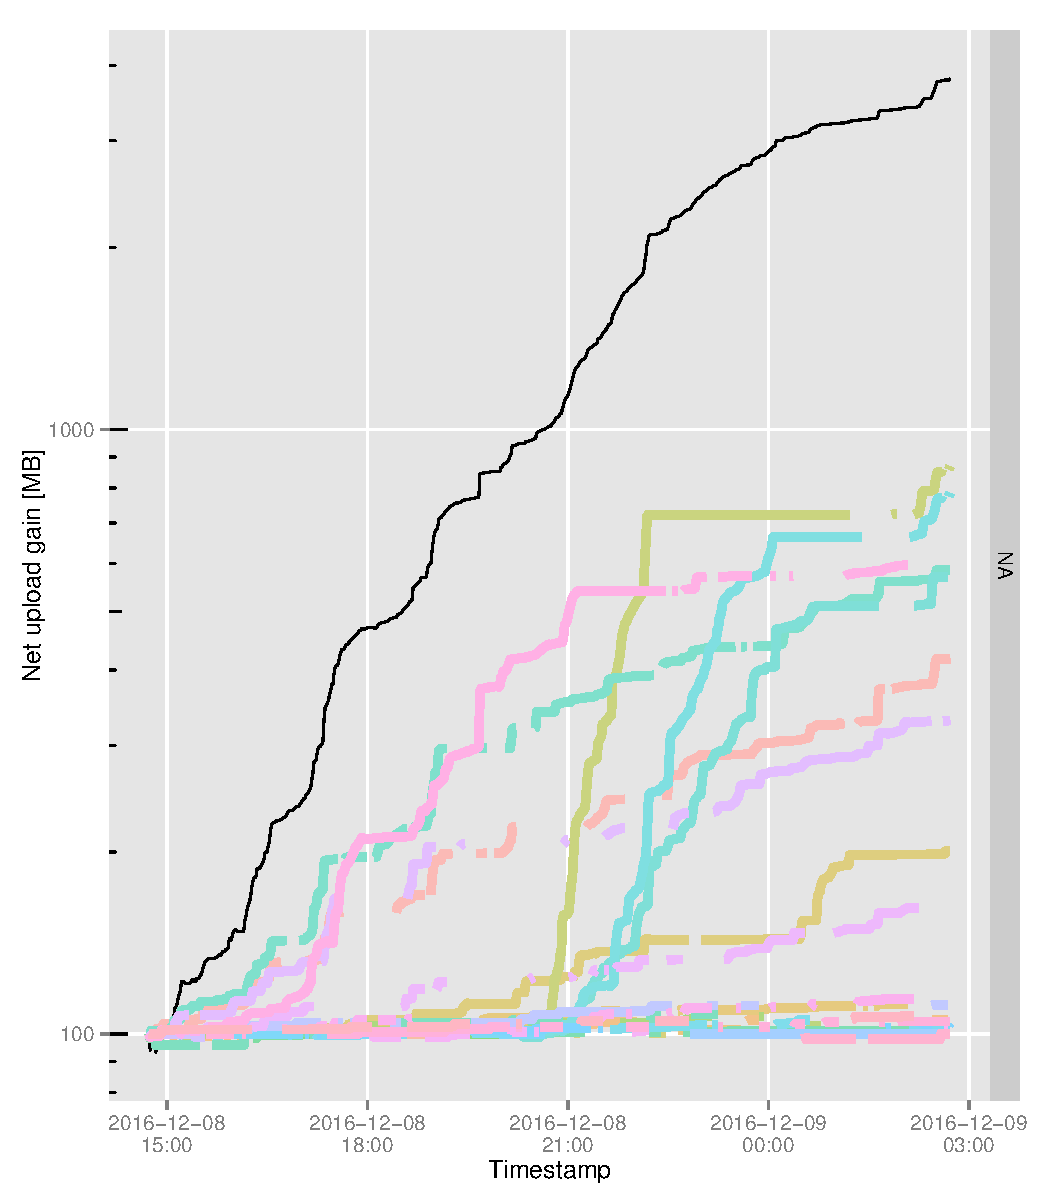
\includegraphics[width=\textwidth]{pics/results/m137.pdf}
		\caption{12 hour old experiment}
	\end{subfigure}
	\caption{New vs old experiments (run in parallel) result on 12 hour}
		\end{adjustwidth}
\end{figure}

\begin{figure}[h!]
	\begin{adjustwidth}{-2.5cm}{}
		\begin{subfigure}[t]{0.7\textwidth}
			\centering
			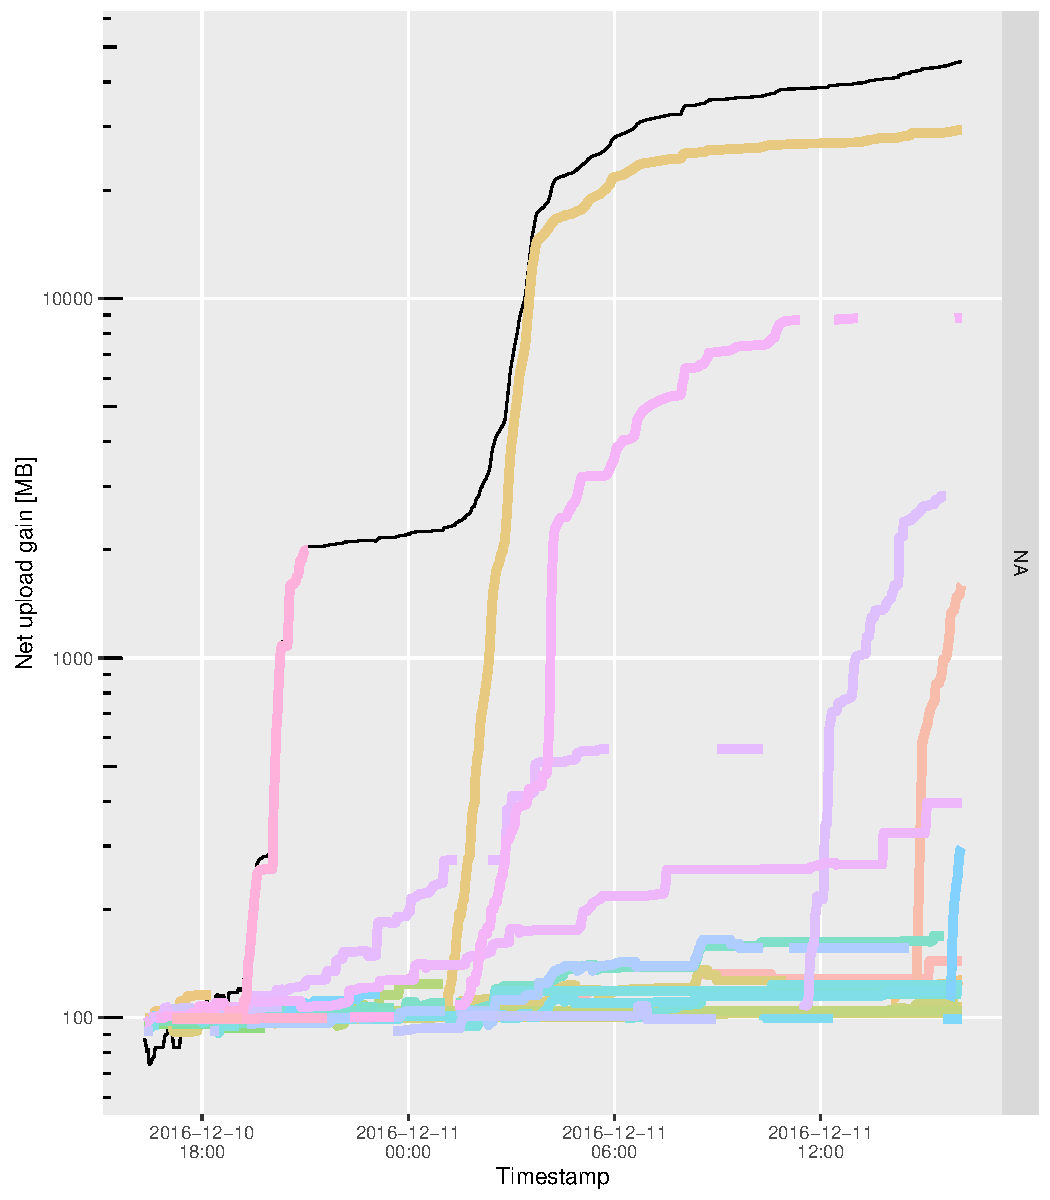
\includegraphics[width=\textwidth]{pics/results/b136.pdf}
			\caption{24 hour new experiment.}
		\end{subfigure}
		~
		\begin{subfigure}[t]{0.7\textwidth}
			\centering
			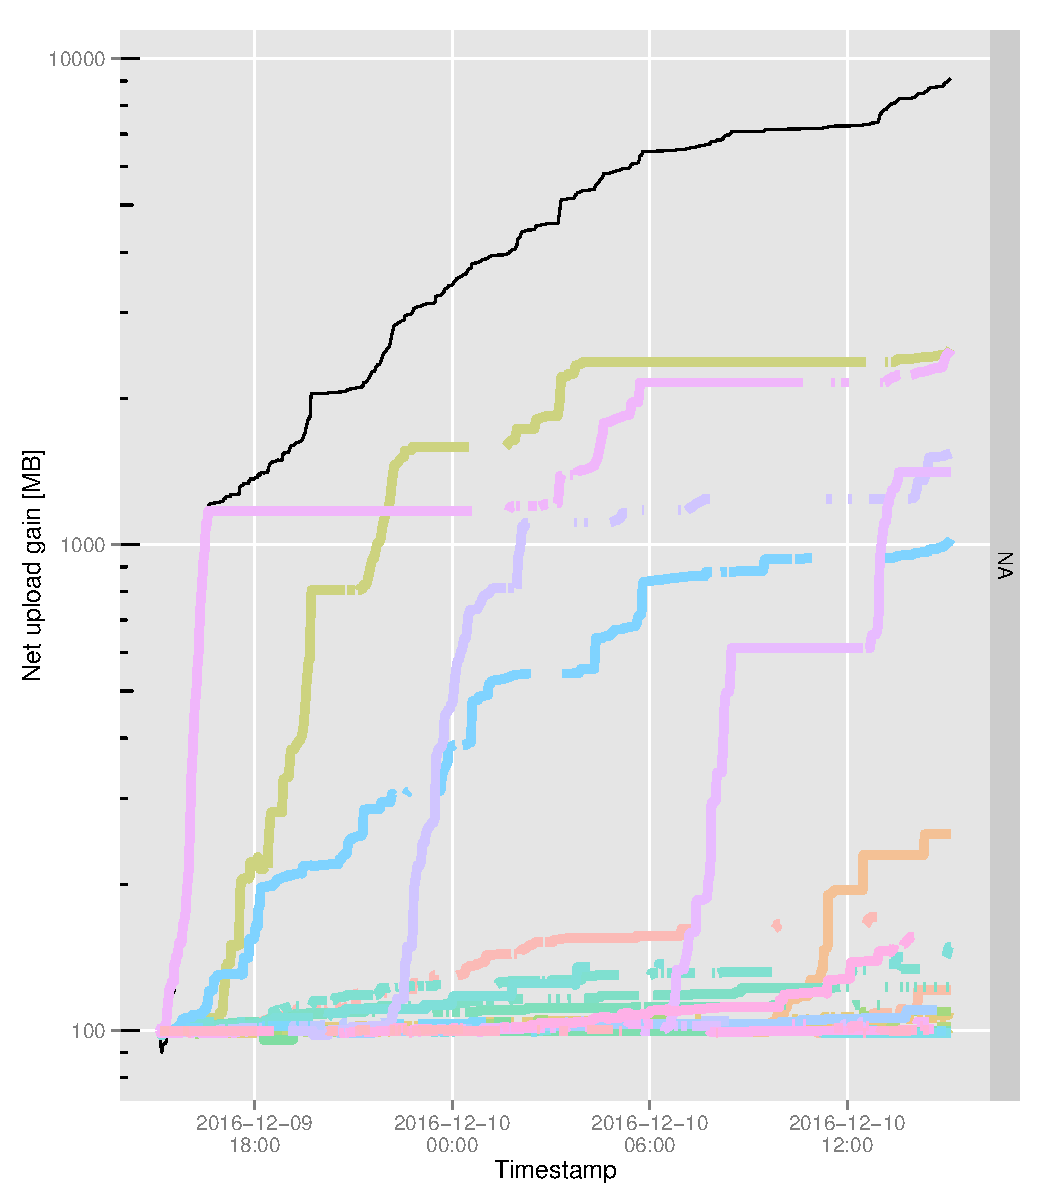
\includegraphics[width=\textwidth]{pics/results/m138.pdf}
			\caption{24 hour old experiment}
		\end{subfigure}
		\caption{New vs old experiments (run separately) result on 24 hour}
	\end{adjustwidth}
\end{figure}

\begin{figure}[h!]
	\begin{adjustwidth}{-2.5cm}{}
		\begin{subfigure}[t]{0.7\textwidth}
			\centering
			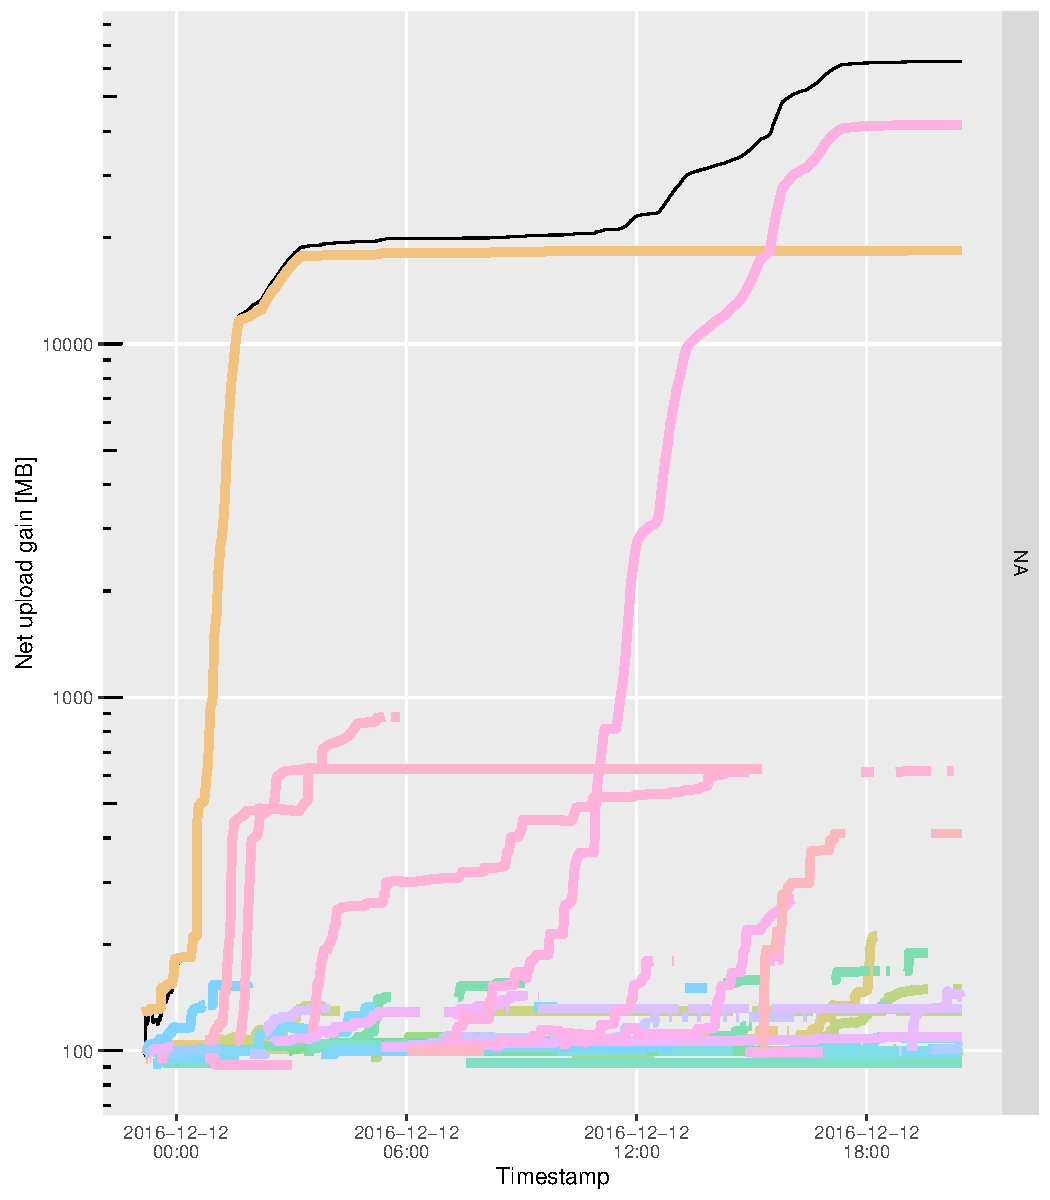
\includegraphics[width=\textwidth]{pics/results/b137.pdf}
			\caption{24 hour new experiment.}
		\end{subfigure}
		~
		\begin{subfigure}[t]{0.7\textwidth}
			\centering
			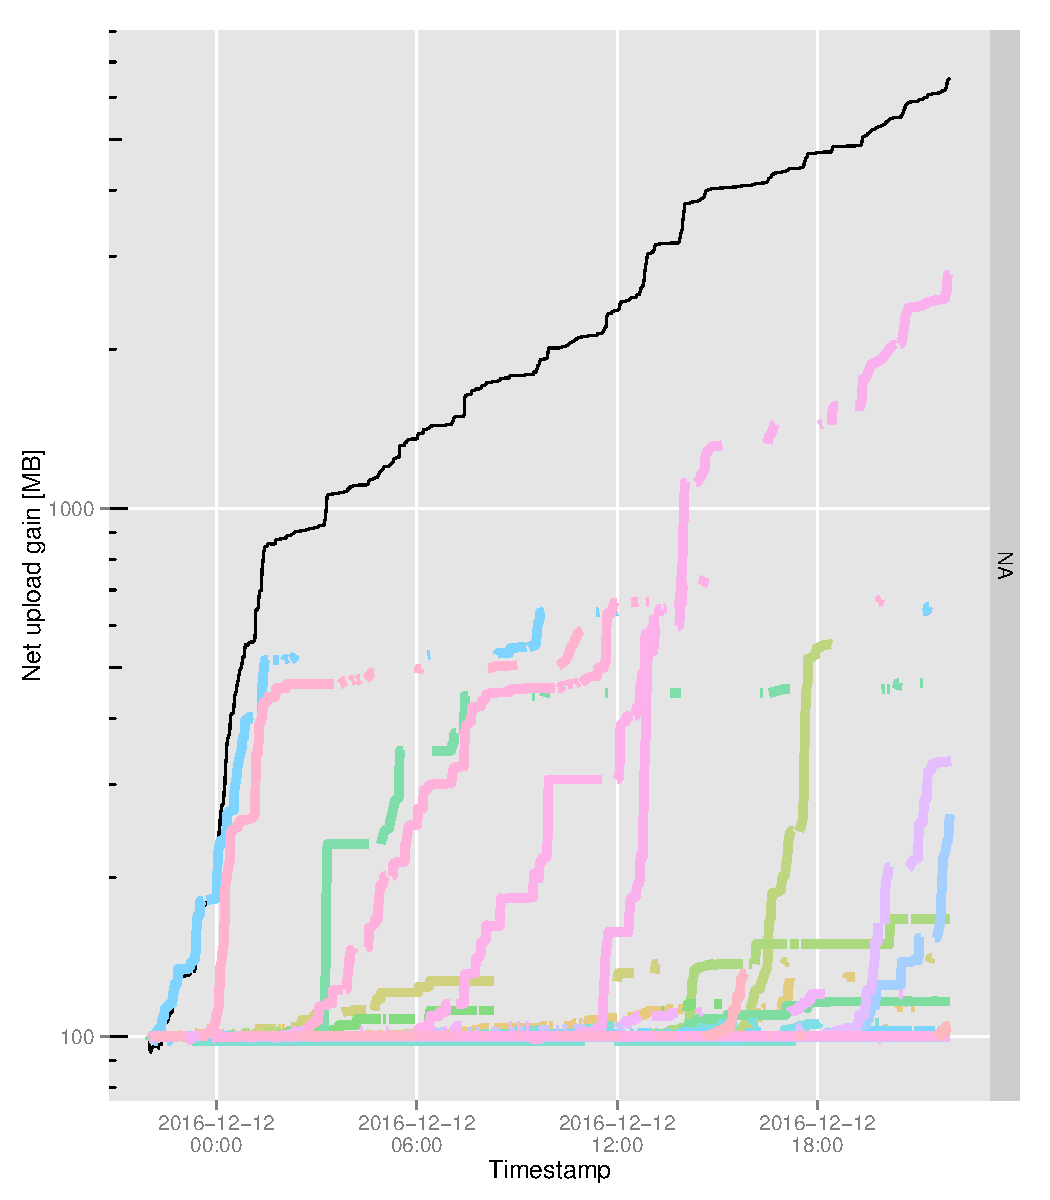
\includegraphics[width=\textwidth]{pics/results/m139.pdf}
			\caption{24 hour old experiment}
		\end{subfigure}
		\caption{New vs old experiments (run in parallel) result on 24 hour}
	\end{adjustwidth}
\end{figure}
%\begin{itemize}
%	\item old one use \textit{net upload gain}. etree.org for two day (48 hour). Test with 1 and half day.
%	\item Best old one is SeederRatio with 5 minute with 1 ratio (gain higher upload gain). Optimal : 3 ratio.
%	\item CM+boost : seederratio, 5 minutes, 3 ratio
%	\item mihai 136 12 hour. runs first. 6dec
%	\item cm 133. 12 hour. runs second. 8dec
%	\item mihai 137, cm 134 : 12 hour. In parallel
%	\item mihai 138 -> cm 136 24h
%	\item mihai 139 & 137 24h par
%\end{itemize}
\clearpage
\section{Priority}
\todo[inline]{WORK ON PROGRESS - Run experiment to find out}
% #50 -> 25k secs : 7 hour
% #50 -> 12h : 
\todo[inline]{temporary graph}
\begin{figure}[h]
	\centering
	\includegraphics[width=\textwidth]{pics/results/tmp_prio_4.png}
	\caption{Download speed of user download activity vs credit mining}
	\label{fig:cmpriomeanagg}
\end{figure}
\begin{figure}[h]
	\centering
	\includegraphics[width=\textwidth]{pics/results/tmp_prio_5.png}
	\caption{Download speed of user download activity only}
	\label{fig:cmpriomean}
\end{figure}

\clearpage
\section{Swarm performance}
\todo[inline]{WORK ON PROGRESS - Waiting for results}
\begin{figure}[h]
	\centering
	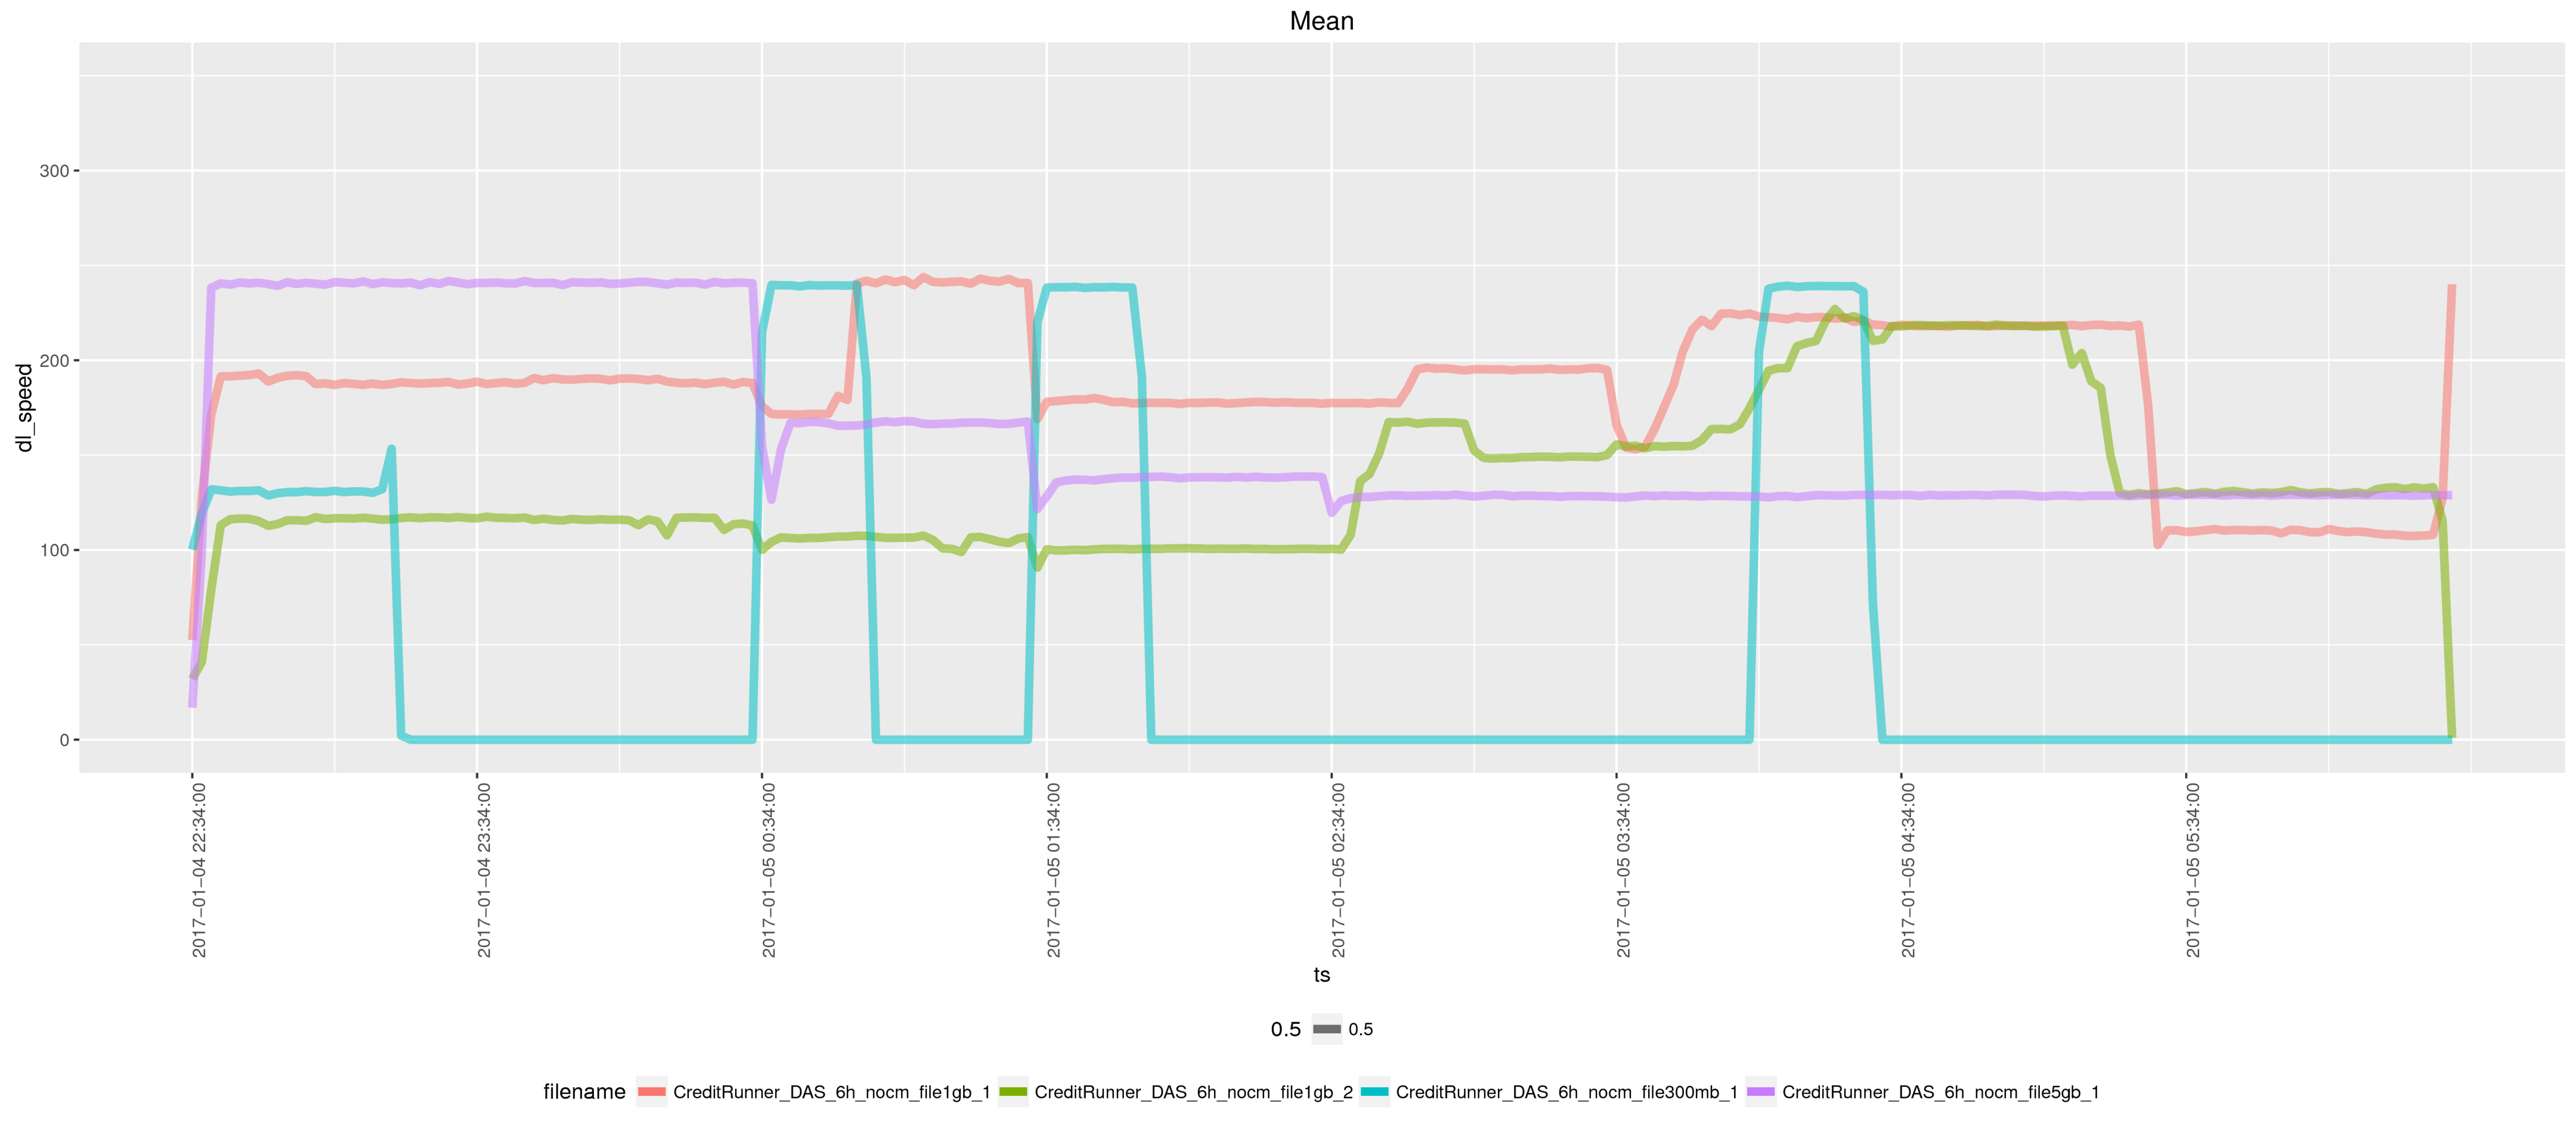
\includegraphics[width=\textwidth]{pics/results/reg_nocm.png}
	\caption{Swarm performance without credit mining}
	\label{fig:swarmnocmperf}
\end{figure}

\begin{figure}[h]
	\centering
	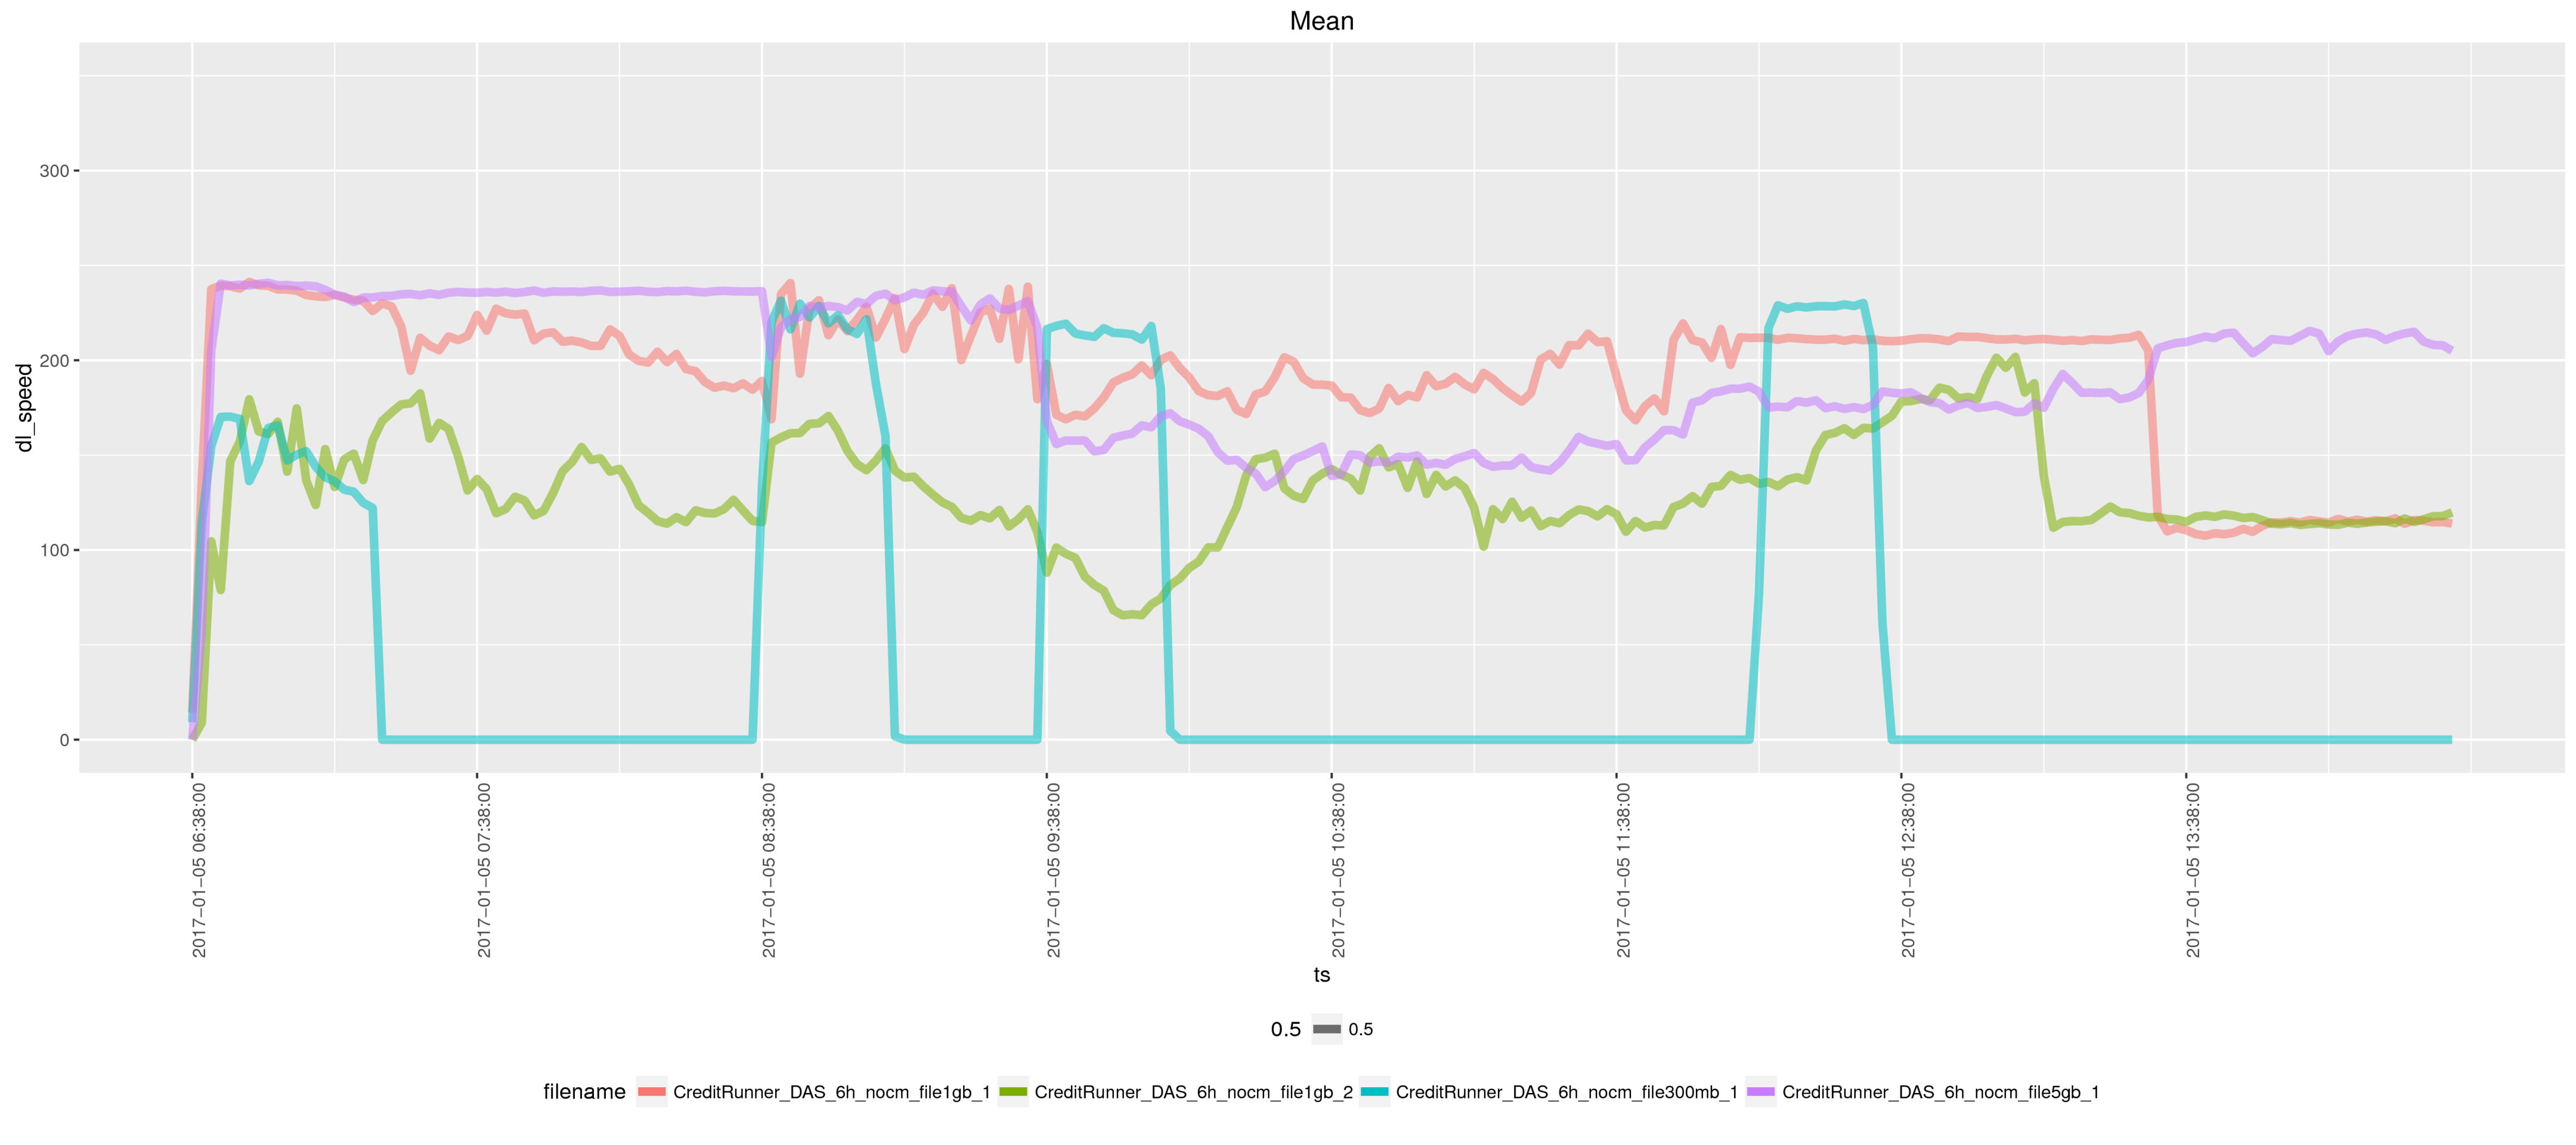
\includegraphics[width=\textwidth]{pics/results/reg_cma.png}
	\caption{Swarm performance with credit mining in the swarm}
	\label{fig:swarmcmperf}
\end{figure}

\begin{figure}[h]
	\centering
	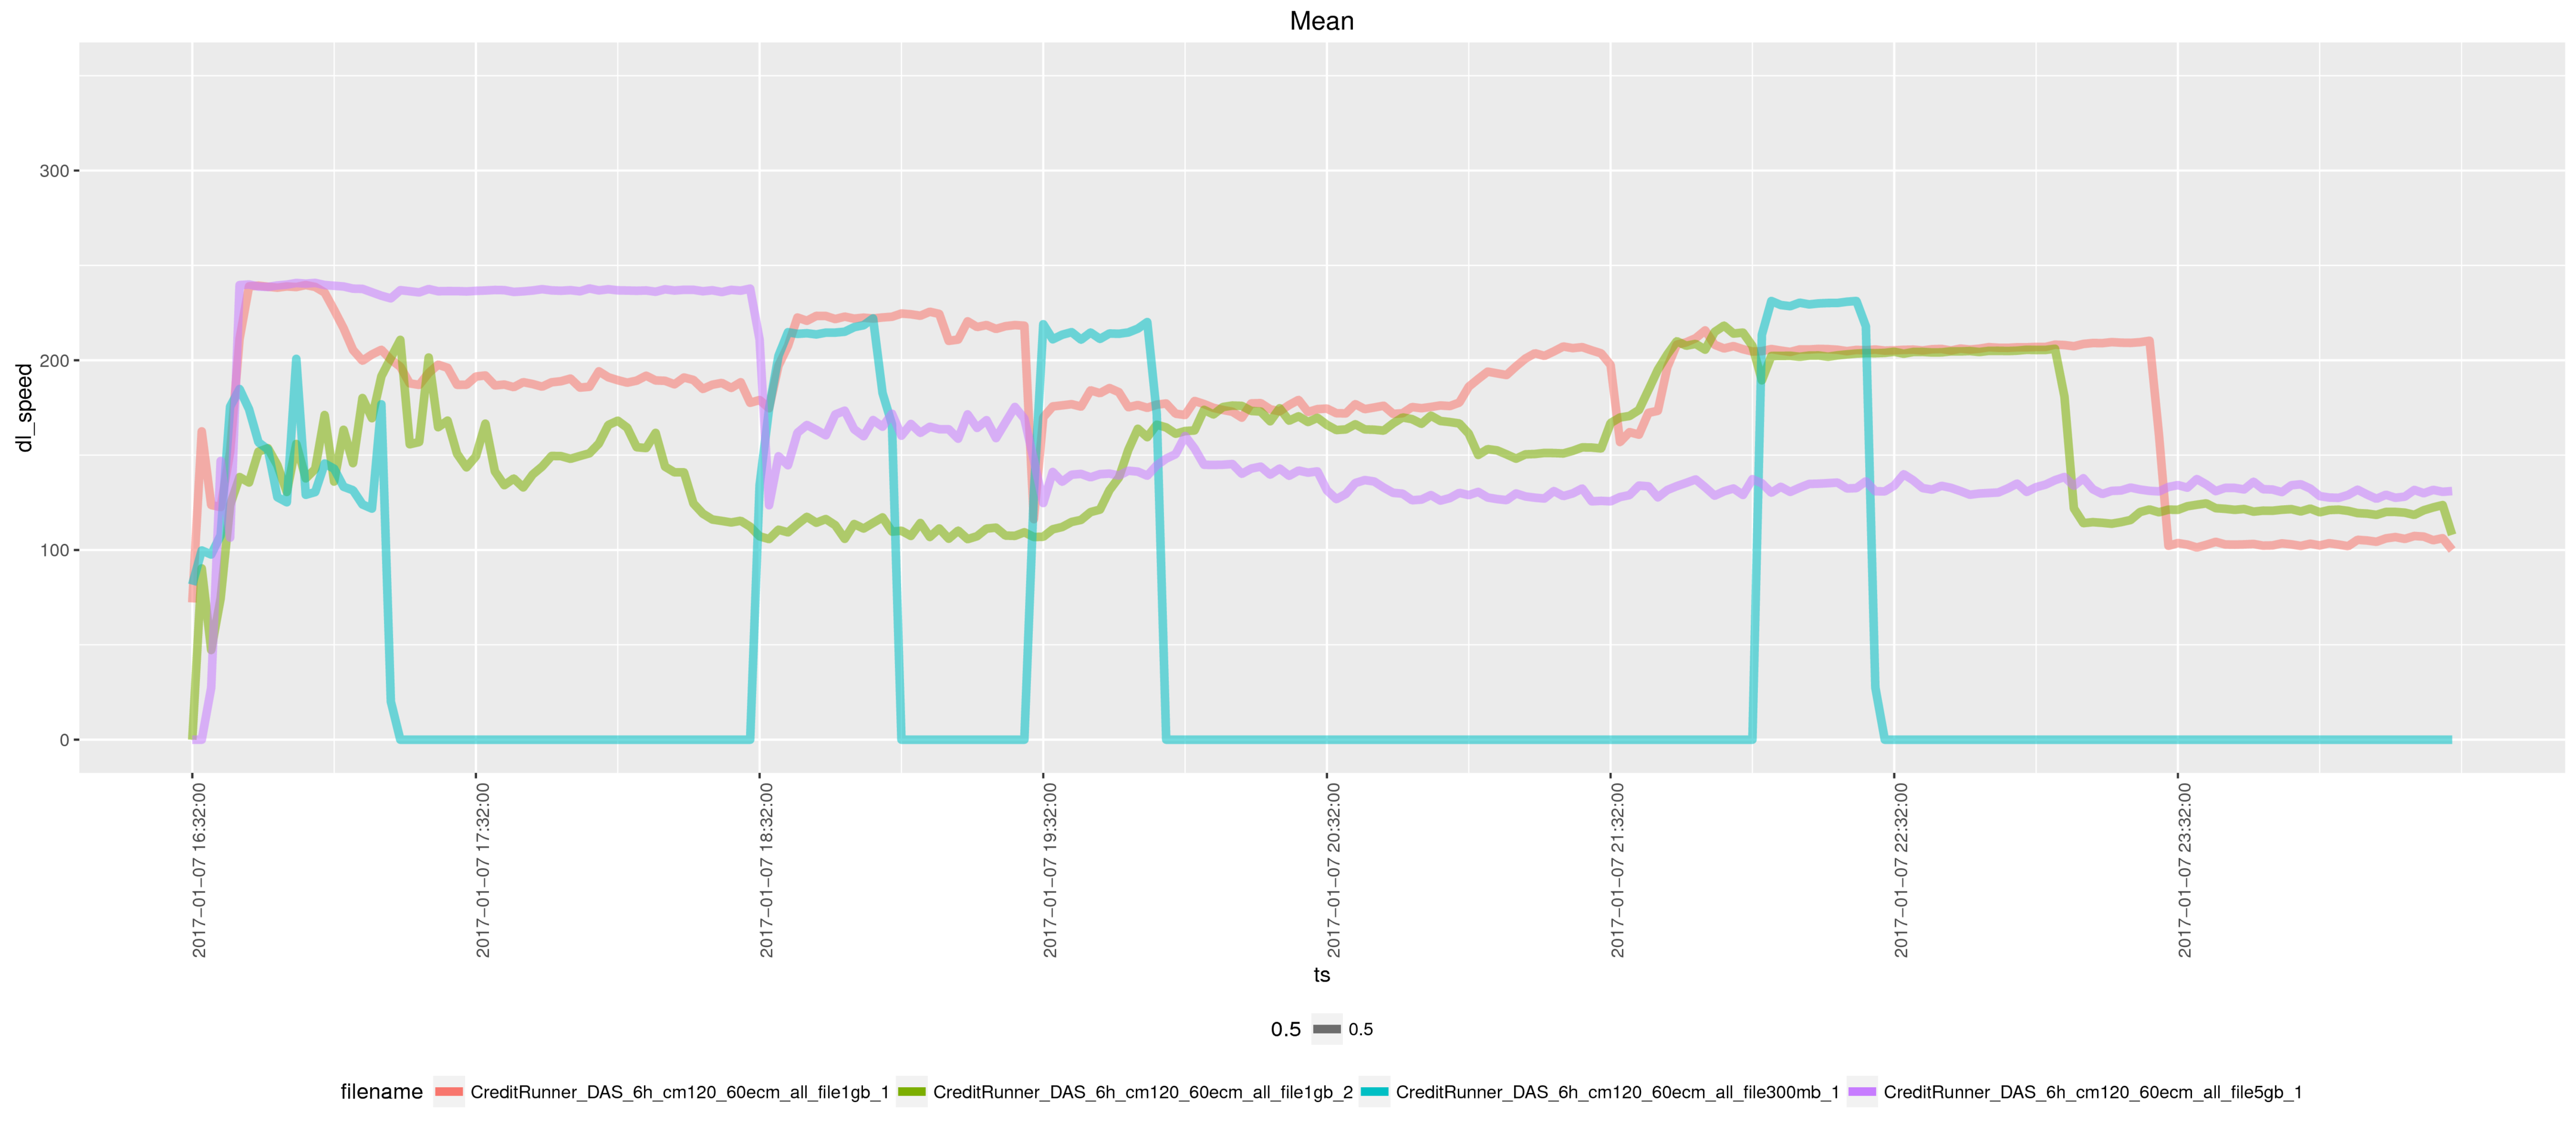
\includegraphics[width=\textwidth]{pics/results/reg_cm+60a.png}
	\caption{Swarm performance with credit mining outside the swarm (60 miners)}
	\label{fig:swarmcm60perf}
\end{figure}

\begin{figure}[h]
	\centering
	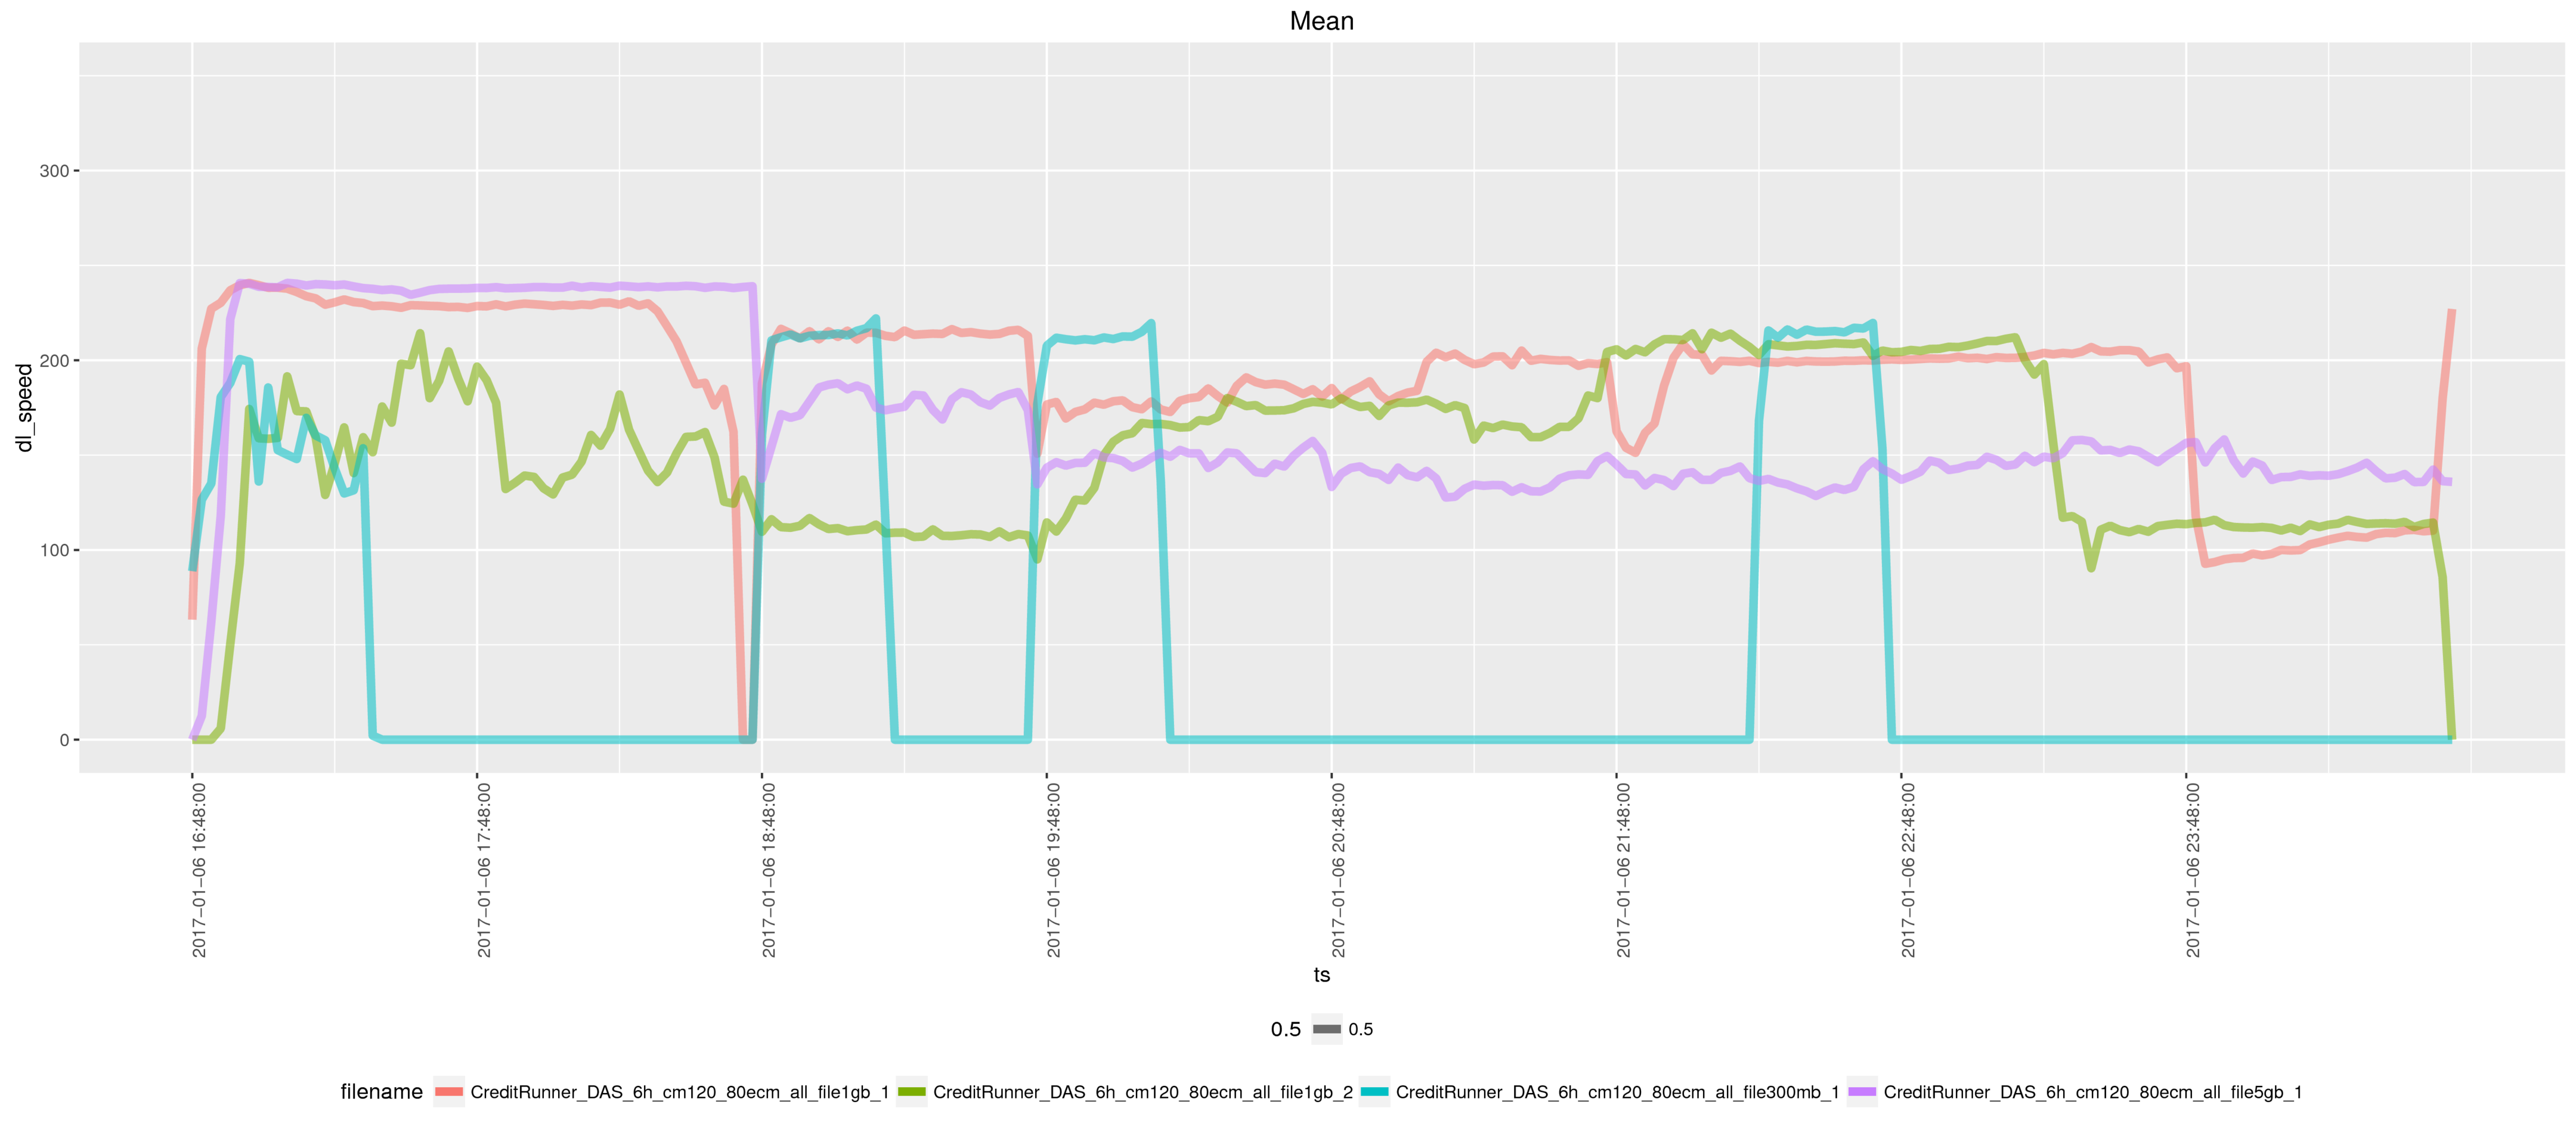
\includegraphics[width=\textwidth]{pics/results/reg_cm+80a.png}
	\caption{Swarm performance with credit mining outside the swarm (80 miners)}
	\label{fig:swarmcm80perf}
\end{figure}

\todo[inline]{single swarm}
\todo[inline]{scoring inside}

\clearpage
\section{Swarm choose}
\begin{table}[h]
	\centering
	\caption{Probability swarm chooser}
	\begin{adjustwidth}{-2.5cm}{}
		\begin{tabular}{|c|p{1.5cm}|p{1.5cm}|p{1.5cm}|p{1.5cm}||c|p{1.5cm}|p{1.5cm}|p{1.5cm}|p{1.5cm}|}
			\hline
			\rowcolor[HTML]{EFEFEF} 
			No. & \textit{sc} top 3 (top 6) & \textit{sr} top 3 (top 6) & \textit{sc} on top session & \textit{sr} on top session & No. & \textit{sc} top 3 (top 6) & \textit{sr} top 3 (top 6) & \textit{sc} on top session & \textit{sr} on top session \\ \hline
			1 & 0  (0) & 0  (0) & 0 & 0 & 19 & 1  (1) & 1  (1) & 1 & 2\\ \hline
			2 & 0  (0) & 1  (1) & 0 & 1 & 20 & 1  (1) & 1  (1) & 2 & 2\\ \hline
			3 & 0  (0) & 1  (1) & 0 & 1 & 21 & 1  (2) & 1  (1) & 2 & 2\\ \hline
			4 & 1  (2) & 1  (1) & 2 & 2 & 22 & 1  (2) & 1  (1) & 2 & 2\\ \hline
			5 & 1  (2) & 1  (1) & 2 & 1 & 23 & 1  (2) & 1  (1) & 2 & 2\\ \hline
			6 & 2  (3) & 1  (1) & 3 & 1 & 24 & 1  (1) & 1  (0) & 2 & 2\\ \hline
			7 & 2  (3) & 1  (1) & 3 & 1 & 25 & 1  (0) & 1  (0) & 2 & 2\\ \hline
			8 & 1  (2) & 1  (1) & 2 & 2 & 26 & 1  (0) & 1  (0) & 1 & 2\\ \hline
			9 & 2  (3) & 1  (1) & 3 & 1 & 27 & 1  (0) & 1  (0) & 1 & 1\\ \hline
			10 & 2  (3) & 1  (1) & 3 & 1 & 28 & 1  (0) & 1  (0) & 1 & 1\\ \hline
			11 & 2  (3) & 1  (1) & 3 & 1 & 29 & 1  (0) & 1  (0) & 1 & 1\\ \hline
			12 & 2  (3) & 1  (1) & 3 & 1 & 30 & 1  (0) & 1  (0) & 1 & 1\\ \hline
			13 & 2  (3) & 1  (1) & 3 & 1 & 31 & 1  (0) & 1  (0) & 1 & 1\\ \hline
			14 & 1  (2) & 1  (1) & 2 & 1 & 32 & 1  (0) & 1  (0) & 1 & 1\\ \hline
			15 & 1  (1) & 1  (1) & 2 & 2 & 33 & 0  (0) & 1  (0) & 0 & 1\\ \hline
			16 & 2  (2) & 1  (1) & 2 & 1 & 34 & 0  (0) & 1  (0) & 0 & 1\\ \hline
			17 & 1  (2) & 1  (1) & 2 & 1 & 35 & 0  (0) & 1  (0) & 0 & 1\\ \hline
			18 & 2  (1) & 1  (0) & 2 & 2 & 36 & 0  (0) & 0  (0) & 0 & 0\\ \hline
		\end{tabular}
	\end{adjustwidth}
\end{table}

Alternative : 

\begin{table}[h]
	\centering
	\caption{Probability swarm chooser (percentage)}
	\begin{adjustwidth}{-2.5cm}{}
		\begin{tabular}{|c|p{1.8cm}|p{1.8cm}|p{1.3cm}|p{1.3cm}||c|p{1.8cm}|p{1.8cm}|p{1.3cm}|p{1.3cm}|}
			\hline
			\rowcolor[HTML]{EFEFEF} 
			No. & \textit{sc} top 3 (top 6) & \textit{sr} top 3 (top 6) & \textit{sc} on top session & \textit{sr} on top session & No. & \textit{sc} top 3 (top 6) & \textit{sr} top 3 (top 6) & \textit{sc} on top session & \textit{sr} on top session \\ \hline
			1 & 0\%(0\%) & 0\%(0\%) & 0\% & 0\% & 19 & 33\%(33\%) & 33\%(33\%) & 33\% & 67\%\\\hline
			2 & 0\%(0\%) & 33\%(33\%) & 0\% & 33\% & 20 & 33\%(33\%) & 33\%(33\%) & 67\% & 67\%\\\hline
			3 & 0\%(0\%) & 33\%(33\%) & 0\% & 33\% & 21 & 33\%(67\%) & 33\%(33\%) & 67\% & 67\%\\\hline
			4 & 33\%(67\%) & 33\%(33\%) & 67\% & 67\% & 22 & 33\%(67\%) & 33\%(33\%) & 67\% & 67\%\\\hline
			5 & 33\%(67\%) & 33\%(33\%) & 67\% & 33\% & 23 & 33\%(67\%) & 33\%(33\%) & 67\% & 67\%\\\hline
			6 & 67\%(100\%) & 33\%(33\%) & 100\% & 33\% & 24 & 33\%(33\%) & 33\%(0\%) & 67\% & 67\%\\\hline
			7 & 67\%(100\%) & 33\%(33\%) & 100\% & 33\% & 25 & 33\%(0\%) & 33\%(0\%) & 67\% & 67\%\\\hline
			8 & 33\%(67\%) & 33\%(33\%) & 67\% & 67\% & 26 & 33\%(0\%) & 33\%(0\%) & 33\% & 67\%\\\hline
			9 & 67\%(100\%) & 33\%(33\%) & 100\% & 33\% & 27 & 33\%(0\%) & 33\%(0\%) & 33\% & 33\%\\\hline
			10 & 67\%(100\%) & 33\%(33\%) & 100\% & 33\% & 28 & 33\%(0\%) & 33\%(0\%) & 33\% & 33\%\\\hline
			11 & 67\%(100\%) & 33\%(33\%) & 100\% & 33\% & 29 & 33\%(0\%) & 33\%(0\%) & 33\% & 33\%\\\hline
			12 & 67\%(100\%) & 33\%(33\%) & 100\% & 33\% & 30 & 33\%(0\%) & 33\%(0\%) & 33\% & 33\%\\\hline
			13 & 67\%(100\%) & 33\%(33\%) & 100\% & 33\% & 31 & 33\%(0\%) & 33\%(0\%) & 33\% & 33\%\\\hline
			14 & 33\%(67\%) & 33\%(33\%) & 67\% & 33\% & 32 & 33\%(0\%) & 33\%(0\%) & 33\% & 33\%\\\hline
			15 & 33\%(33\%) & 33\%(33\%) & 67\% & 67\% & 33 & 0\%(0\%) & 33\%(0\%) & 0\% & 33\%\\\hline
			16 & 67\%(67\%) & 33\%(33\%) & 67\% & 33\% & 34 & 0\%(0\%) & 33\%(0\%) & 0\% & 33\%\\\hline
			17 & 33\%(67\%) & 33\%(33\%) & 67\% & 33\% & 35 & 0\%(0\%) & 33\%(0\%) & 0\% & 33\%\\\hline
			18 & 67\%(33\%) & 33\%(0\%) & 67\% & 67\% & 36 & 0\%(0\%) & 0\%(0\%) & 0\% & 0\%\\\hline
		\end{tabular}
	\end{adjustwidth}
\end{table}

Statistics (scoring vs seeder ratio): 
\begin{enumerate}
	\item Strictly larger Top 3  : 9 (25 \% better)
	\item Strictly larger Top 6  : 18 (50 \% better)
	\item Strictly larger top session  : 11
	\item larger or equal Top 3  : 32 (cover 88 \%)
	\item larger or equal Top 6  : 35 (cover 97 \%)
	\item larger or equal top session  : 30
\end{enumerate}